\documentclass[a4paper,12pt]{article}

\usepackage[top= 27mm, bottom=27mm, left=25mm, right=25mm]{geometry}

\usepackage[english,serbianc]{babel}
\usepackage[OT1, OT2]{fontenc}
\usepackage{epstopdf}
\usepackage{graphicx}
\usepackage{enumerate}
\usepackage{amsmath,amsthm,amssymb}
\usepackage{hyperref}
\usepackage{multicol}


\newcommand{\Lat}{\fontencoding{OT1}\selectfont} 
\newcommand{\Cir}{\fontencoding{OT2}\selectfont} 
\newcommand{\HRule}{\rule{\linewidth}{0.5mm}}

\renewcommand{\arctg}{\operatorname{arctg}}
\renewcommand{\tg}{\operatorname{tg}}


\begin{document}

\begin{titlepage}

\center
\textup{\Large Univerzitet u Beogradu\\Matematichki fakultet}\\[1.5cm]


\vfill
\vfill
\vfill

\textup{\Large Seminarski rad iz Programskih paketa u matematici}\\[0.4cm]
\HRule \\[0.4cm]
{ \huge \bfseries Reshenja zadataka sa prijemnih ispita}\\[0.4cm]
\HRule \\[8.5cm]

\begin{minipage}{0.4\textwidth}
\begin{flushleft}
\large
\emph{Autor:}\\
\textup Ivana Jankic1\\
Broj indeksa: 4/2013
\end{flushleft}
\end{minipage}
\hfill
\begin{minipage}{0.4\textwidth}
\begin{flushright}
\large
\emph{Predmetni asistent:} \\
\textup Matej Milic1evic1\\
\end{flushright}
\end{minipage}\\[2cm]

{\large \today}\\[3cm] 
\end{titlepage}


%sadrzaj
\tableofcontents

\newpage



\section{Prijemni ispit iz 2016. godine}



\subsection{Zadaci}

\begin{enumerate}[1.]
\item Kada je 25\% kante prazno, ona sadrzhi 25 litara vode vishe nego kada je 25\% kante puno. Koliko litara vode sadrzhi puna kanta?
{\Lat
\begin{multicols}{5}
\begin{enumerate}[A)]
\item 25 \item 33 \item 50 \item 75 \item 90
\end{enumerate}
\end{multicols}
}
\item Dvocifreni zavrshetak prirodnog broja $a$ je 16. Ako broj $a$ nije deljiv sa 8, tada je cifra jedinica broja $3a/4$ jednaka:
{\Lat
\begin{multicols}{5}
\begin{enumerate}[A)]
\item 0 \item 2 \item 5 \item 7 \item 8
\end{enumerate}
\end{multicols}
}
\item Koliko ima prirodnih brojeva manjih od 1000000 koji su deljivi tachno jednim od brojeva 11 i 13?
{\Lat
\begin{multicols}{5}
\begin{enumerate}[A)]
\item 6993 \item 153846 \item 160839 \item 167832 \item 993006
\end{enumerate}
\end{multicols}
}

\item Najvec1i koeficijent polinoma $(2x + 1)^{10} $ jednak je:
{\Lat
\begin{multicols}{5}
\begin{enumerate}[A)]
\item 120 \item 11520 \item 13440 \item 15360 \item 16480
\end{enumerate}
\end{multicols} 
}

\item Brojevi 2, $\sqrt{6} - \sqrt{2} $ i $4 - 2\sqrt{3}$ chine prva tri chlana:
{\Lat
\begin{enumerate}[A)] 
\item { \Cir aritmetichkog, ali ne i geometrijskog niza }
\item { \Cir geometrijskog, ali ne i aritmetichkog niza }
\item { \Cir i aritmetichkog i geometrijskog niza }
\item { \Cir ni aritmetichkog ni geometrijskog niza }
\item { \Cir niza sa opshtim chlanom $a_n = 4 - 2\sqrt{n} $ }
\end{enumerate}
}
\item Data je jednachina $\left(\frac{1 + ix}{1 - ix}\right)^2 = i $, gde je $x$ realna nepoznata. Broj reshenja ove jednachine u intervalu $(0,1/2)$ je:
{\Lat
\begin{multicols}{5}
\begin{enumerate}[A)]
\item 0 \item 1 \item 2 \item 4 \item $\infty$
\end{enumerate}
\end{multicols}
}

\item Ako su $x_1$ i $x_2$ reshenja jednachine $x^2 - x + 15 = 0$, tada je $x_1^3 + x_2^3 - 2x_1^2 - x_2^2 + x_1x_2 + 2x_1 + x_2 -15 $ jednako:
{\Lat
\begin{multicols}{5}
\begin{enumerate}[A)]
\item 1 \item 87 \item 31 \item 16 \item $-14$
\end{enumerate}
\end{multicols}
}

\item Ako su $a$ i $b$ realni brojevi takvi da polinom  $x^4 + ax^3 -ax +b $ daje ostatak $2x+4$  pri deljenju polinomom $x^2 + 2x+ 1$, tada je $ab$ jednako:
{\Lat
\begin{multicols}{5}
\begin{enumerate}[A)]
\item 1 \item 2 \item 3 \item 4 \item 5
\end{enumerate}
\end{multicols}
}

\item Date su funkcije  $ f_1(x) = \ln \frac{1 + \sin{x}}{1 - \sin{x}}$ , $ f_2(x) = \arcsin{x} \cdot \arctg{x} $, $ f_3(x) = \sin{x} + \cos{x} $ i $f_4(x) = \frac{\ln{x^2}}{\sqrt[3]{x}} $. Ako sa $p$ oznachimo broj parnih, a sa $n$ broj neparnih medju ovim funkcijama, tachan je iskaz:
{\Lat
\begin{multicols}{3}
\begin{enumerate}[A)]
\item $p = 1$ i $n = 1$ \item $p = 2$ i $n = 2$ \item $p = 2$ i $n = 1$ \item $p = 1$ i $n = 2$ \item $p = 1$ i $n = 0$
\end{enumerate}
\end{multicols}
}



\item Za koje vrednosti realnog parametra $a$ jednachina $||x-3|-1|=a$ ima tachno tri realna reshenja:
{\Lat
\begin{multicols}{5}
\begin{enumerate}[A)]
\item $-1$ \item 0 \item 1 \item 2 \item 3
\end{enumerate}
\end{multicols}
}


\item Funkcija $f$ je zadata sa $f(x) = \frac{ax +b}{cx+d} $, gde su $a,b,c$ i $d$ realni brojevi. Ako je $f(0) = 1$,  $f(1) = 0$ i  $f(2) = 3$, koliko je  $f(3)$?
{\Lat
\begin{multicols}{5}
\begin{enumerate}[A)]
\item $-1$ \item $\frac{3}{2}$ \item 5 \item 2 \item 3
\end{enumerate}
\end{multicols}
}


\item Broj reshenja sistema jednachina 
\par $(x^{2} - 1)(2x -3y + 4z) = 0$
\par $4x + 5y +8z = -2$
\par $3x + y + 6z = 44$
\par u skupu realnih brojeva je: 
{\Lat
\begin{multicols}{5}
\begin{enumerate}[A)]
\item 0 \item 1 \item 2 \item 3 \item $\infty$
\end{enumerate}
\end{multicols}
}

\item Ako za realne brojeve $x$  i $y$ vazhi $7 \cdot 3^{x} - 5 \cdot 2^{y} = 23$ i $2 \cdot 3^{x} + 3 \cdot 2^{y} = 42$, onda je zbir $x + y$ jednak:
{\Lat
\begin{multicols}{5}
\begin{enumerate}[A)]
\item 7 \item 2 \item 3 \item 4 \item 5
\end{enumerate}
\end{multicols}
}


\item Proizvod svih reshenja jednachine $ \log_{36} x^{2} + \log_6 (x + 5) -1 = 0$ je :
{\Lat
\begin{multicols}{5}
\begin{enumerate}[A)]
\item $-36$ \item $-6$ \item 1 \item 12 \item 6
\end{enumerate}
\end{multicols}
}


\item Broj celobrojnih reshenja nejednachine $\sin{x} < \lvert \cos{x} \rvert $ u intervalu $[ 0,8] $ jednak je: 
{\Lat
\begin{multicols}{5}
\begin{enumerate}[A)]
\item 4 \item 5 \item 6 \item 7 \item 8
\end{enumerate}
\end{multicols}
}

\item Tachke $M,N$ i $P$ su sredishta tri medjusobno mimoilazne ivice kocke. Ako je duzhina ivice $4\mathrm{\ cm}$, povrshina trougla $MNP$ je:
{\Lat
\begin{multicols}{5}
\begin{enumerate}[A)]
\item $8\sqrt{2}\mathrm{\ cm}^2$ \item $\sqrt{2}\mathrm{\ cm}^2$ \item $8\sqrt{3}\mathrm{\ cm}^2$ \item $8\mathrm{\ cm}^2$ \item $6\sqrt{3}\mathrm{\ cm}^2$
\end{enumerate}
\end{multicols}
}

\item Oko kruzhnice opisan je chetvorougao $ABCD$ povrshine $90cm^2$. Ako je zbir duzhina naspramnih stranica $AB$ i $CD$ jednak $15\mathrm{\ cm}$, duzhina poluprechnika kruzhnice je: 
{\Lat
\begin{multicols}{5}
\begin{enumerate}[A)]
\item $6\mathrm{\ cm}$ \item $5\sqrt{2}\mathrm{\ cm}$ \item $6\sqrt{3}\mathrm{\ cm}$ \item $3\sqrt{3}\mathrm{\ cm}$ \item $3\mathrm{\ cm}$
\end{enumerate}
\end{multicols}
}

\item Date su dve koncentrichne kruzhnice i duzh $AB$ koja je tetiva kruzhnice vec1eg, a tangenta na kruzhnicu manjeg poliprechnika. Ako je $AB = 6$, onda je povrshina prstena izmedju datih kruzhnica jednaka: 
{\Lat
\begin{multicols}{5}
\begin{enumerate}[A)]
\item $12\pi$  \item $9\pi$ \item $\pi$ \item 9 \item $6\pi$
\end{enumerate}
\end{multicols}
}

\item Povrshina kvadrata chije su dve stranice na pravima $2x + y - 3 = 0$, $2x +y -8 = 0$ je :
{\Lat
\begin{multicols}{5}
\begin{enumerate}[A)]
\item $2\sqrt{3}$  \item 5 \item 4 \item 6 \item $3\sqrt{2}$
\end{enumerate}
\end{multicols}
}

\item Duzhine stranica oshtrouglog trougla su $a = 60$, $ b = 52$ i $c$, a velichine odgovarajuc1ih uglova su $\alpha,\beta  $ i $\gamma $. Ako je $\sin{\alpha } = \frac{12}{13}$, onda je $\sin{\gamma }$ jednak:
{\Lat
\begin{multicols}{5}
\begin{enumerate}[A)]
\item $\frac{56}{65}$  \item $\frac{56}{63}$ \item $\frac{39}{65}$ \item $\frac{39}{63}$ \item $\frac{63}{65}$
\end{enumerate}
\end{multicols}
}

\end{enumerate}






\newpage

\subsection{Reshenja}
\begin{enumerate}[1.]

\item 25\% kante je prazne je ekvivalentno sa tim da je 75\% kante puno. Obelezhimo sa $x$ zapreminu kante sa vodom. Prevedimo sada tekst zadatka u matematichki zapis:
\par Kada je 25\% kante prazno, ona sadrzhi 25 litara vode vishe nego kada je 25\% kante puno.
\par 75\% od $x$ umanjen sa 25 litara je isto sto i 25\% od $x$.
\par Matematichki : $ 0.75 \cdot x - 25 = 0.25 \cdot x$
\par Daljim reshavanjem ove jednachine dobijamo: $ 0.5 \cdot x = 25$. Ako obe strane pomozhimo sa brojem 2 dobijamo: $x = 50$, te je reshenja zadatka 50 litara. \textbf{Odgovor je pod $C$.}

\item Dvocifreni zavrshetak prirodnog broja $a$ je 16, matematichki zapisano $ a \equiv 16 \pmod{100}$. Znamo da 8 ne sme da deli $a$, dok po tekstu zadatka zakljuchujemo da 4 mora da deli $a$. Uradimo zadatak peshaka, ispishimo sve dvocifrene i trocifrene brojeve kod kojih vazhi gornja relacija. Krenuc1emo od 16 do 916.
\par 16 - ne mozhe jer je deljivo sa 8.
\par 116 je kandidat za $a$.
\par 216 - ne mozhe jer je deljivo sa 8.
\par 316 je kandidat za $a$.
\par 416 - ne mozhe jer je deljivo sa 8.
\par 516 je kandidat za $a$.
\par 616 - ne mozhe jer je deljivo sa 8.
\par 716 je kandidat za $a$.
\par 816 - ne mozhe jer je deljivo sa 8.
\par 916 je kandidat za $a$.
\par Posmatrajmo sada kandidate, svi su deljivi sa 4. Podelimo ih sve sa 4 i dobijamo redom : 29, 79, 129, 179, 229. Poshto nas zanima samo cifra jedinice broja $3a/4$, vec1 odavde mozhemo da zakljuchimo da c1e to biti $9 \cdot 3 \pmod{10}$ to jest broj 7. \textbf{Odgovor je pod $D$.}

\item Brojeve koje posmatramo pripadaju skupu $ \{n\in \mathbb{N} : n < 1 000 000 = 10^{6}\} $. Posmatrajmo skupove $A = \{ m \in \mathbb{N} : 11\ |\ m\mbox{\ i\ } m < 10^{6}\}$, $B = \{ m \in \mathbb{N} : 13\ |\ m\mbox{\ i\ } m < 10^{6}\}$ i $C = \{ m \in \mathbb{N} : 11 \cdot 13\ |\ m\mbox{\ i \ } m < 10^{6}\}$. $A$ je skup svih brojeva deljivih sa 11, $B$ je skup svih brojeva deljivih sa 13 i $C$ skup svih brojeva deljivih sa 11 i 13. Poshto se u skupu $A$ nalaze brojevi deljivi i sa 13, a u $B$ se nalaze brojevi koji su deljivi i sa 11, reshenje predstavlja $\lvert A \rvert + \lvert B \rvert  - 2 \cdot \lvert C \rvert $, gde $ \lvert A \rvert $ predstavlja kardinalnost skupa A. Izrachunajmo sada kardinalnosti skupova :
\par $ \lvert A \rvert = \left\lfloor \frac{10^{6}}{11}\right\rfloor   = 90909$  
\par  $ \lvert B \rvert = \left\lfloor \frac{10^{6}}{13}\right\rfloor   = 76923$
\par  $ \lvert C \rvert = \left\lfloor \frac{10^{6}}{11 \cdot 13}\right\rfloor = \left\lfloor \frac{10^{6}}{143}\right\rfloor  = 6993$  
\par Te je reshenje $ 90909 + 76923 - 2 \cdot 6993  = 153846$. \textbf{Odgovor je pod $B$.}

\item Koeficijent uz k-ti chlan se rachuna pomoc1u formule $\binom{n}{k}2^k1^{n-k}$, shto je u ovom sluchaju isto shto i $\binom{n}{k}2^{k} $. Sada trazhimo $ k \leq 10$ takvo da je gornji izraz maksimalan. Znamo da $\binom{n}{k}$ daje koeficijente simetrichne u odnosu na $\frac{n + 1}{2} $, pa uochavamo da ce maksimalno biti za $ k \geq \left\lceil \frac{n + 1}{2}\right\rceil   = 6$. Nadjimo sada koeficijente za $ 6 \leq k \leq 10$ : 
\par $\binom{10}{6}\cdot 2^{6} = 210 \cdot 2^{6} = 6720 $
\par $\binom{10}{7}\cdot 2^{7} = 120 \cdot 2^{7} = 15360 $
\par $\binom{10}{8}\cdot 2^{8} = 45 \cdot 2^{8} =  11520$
\par $\binom{10}{9}\cdot 2^{9} = 10 \cdot 2^{9} = 5120 $
\par $\binom{10}{10}\cdot 2^{10} = 1 \cdot 2^{10} = 1024 $
Vidimo da je za $k = 7$ koeficijent najvec1i i iznosi 15360. \textbf{Odgovor je pod $D$.}

\item Ochigledno je da niz nije aritmetichki te odgovori po A i C otpadaju. Proverimo da li je odgovor pod E. Da li su to chlanovi niza $a_n = 4 - 2\sqrt{n} $. Rachunajmo $a_1 = 4-2 = 2$, $a_2 = 4 - 2\sqrt{2}$ - a ovaj broj nije medju trazhenima. Ostalo je josh proveriti da nije geometrijski niz. Pretpostavimo da jeste, nadjimo sada koeficijent geometrijske progresije $q$ :
\par Znamo da je geomerijski niz oblika $b, bq, bq^2, bq^3$ itd. Te $q$ mozhemo nac1i kada dva uzastopna chlana niza podelimo. Poshto je prvi chlan ceo broj, podelic1emo drugi chlan sa prvim : $ \frac{\sqrt{6} - \sqrt{2}}{2} = \frac{\sqrt{2} \cdot (\sqrt{3} - 1)}{2} =\frac{\sqrt{2}}{2} \cdot (\sqrt{3} - 1) $ i to c1e biti $q$. Sada ostaje da proverimo da li trec1i chlan niza pripada geometrijskom nizu chija prva dva chlana su 2 i $\sqrt{6} - \sqrt{2}$. Dovoljno je da pomnozhimo drugi chlan sa $q$ i da vidimo da li je jednak trec1em, ili da podelimo trec1i i drugi i da vidimo da li je jednak $q$. Uradic1emo prvu varijantu : $(\sqrt{6} - \sqrt{2}) \cdot \frac{\sqrt{2}}{2} \cdot (\sqrt{3} - 1) = \sqrt{2} \cdot (\sqrt{3} - 1) \cdot \frac{\sqrt{2}}{2} \cdot (\sqrt{3} - 1) = \sqrt{2} \cdot \frac{\sqrt{2}}{2} \cdot (\sqrt{3} - 1)^2 = 1 \cdot (3 - 2\sqrt{3} + 1) = 4 - 2\sqrt{2}$ shto i jeste trec1i chlan niza, te je on geometrijski. \par \textbf{Odgovor je pod $B$.}

\item Reshavamo jednachinu $\left(\frac{1 + ix}{1 - ix}\right)^2 = i $
\par $\left(\frac{1 + ix}{1 - ix}\right)^2 =\frac{1 +2ix -x^2}{1 -2ix - x^2} = i $, pomnozhimo je sa $1 - 2ix -x^2$ (koji je uvek razlichit od 0, jer je $x$ realan broj) i dobijamo:
\par $1 +2ix -x^2 = i(1 - 2ix -x^2)$ prebacimo sada sve na levu stranu i sredimo
\par $-(1-i)x^2 -(2-2i)x + (1-i) = 0$
\par $-(1-i)x^2 -2(1-i)x + (1-i) = 0$ podelimo sa $-(1-i)$ i dobijamo
\par $x^2 +2x -1 = 0$, proverimo da li je diskriminanta vec1a ili jednaka od 0, shto i jeste.
\par Koristec1i formulu za nalazhenje korena binoma dobijamo: $x_{1,2} = \frac{-2 \pm \sqrt{4 + 4}}{2} = \frac{-2 \pm 2\sqrt{2}}{2} = -1 \pm \sqrt{2}$
\par Znamo da je $\sqrt{2} = 1.41$ te je reshenje iz intervala $(0,1/2)$ samo $-1 + \sqrt{2}$.
\par \textbf{Odgovor je pod $B$.}

\item Ovo se mozhe uraditi na dva nachina, jedan koji je jako rachunski zahtevan sa velikom verovatnoc1om da c1e se negde pogreshiti ili na pametan i elegantan nachin. Ovaj prvi nec1u raditi ali je ochigledno da se odnosi na nalazhenje korena jednachine $x^2 - x + 15 = 0$ i onda ih zameniti u izraz i rachunati. Ali ako dobro pogledamo tu jednachinu videc1emo da su njeni koreni kompleksni brojevi, i ne samo to nego je i izraz sa korenom. Odatle se vec1 vidi da bi taj nachin bio najgori moguc1i. Drugi nachin koji mozhemo sada nazvati i jedini je da se setimo \footnote{ Fransoa Vijet ({\Lat Fran\c{c}ois Vi\`{e}te, 1540---1603 }), francuski matematichar.}{Vijetovih} veza za kvadratne jednachine:
\par Za jednachinu oblika $ax^2 + bx + c = 0$, gde su $x_1$ i $x_2$ koreni vazhi $x_1 + x_2 = \frac{-b}{a}$ i $x_1 \cdot x_2 = \frac{c}{a}$
\par Ideja je sledec1a da izraz sredimo tako da bismo mogli da primenimo Vijetove veze. Sredic1emo ga tako shto c1emo odredjene delove rastavljati na chinioce korisitec1i fromule za trinome i binome.
\par $x_1^3 + x_2^3 - 2x_1^2 - x_2^2 + x_1x_2 + 2x_1 + x_2 -15 = ?$
\par $x_1^3 + x_2^3$ c1emo rastaviti na $(x_1 + x_2)(x_1^2 -x_1x_2 + x_2^2 )$
\par Grupisac1emo $-2x_1^2 +2x_1 = -2(x_1^2 -x_1)$ i $-x_2^2 +x_2 = - (x_2^2 -x_2)$, jer te vrednosti znamo iz kvadratne jednachine. Kako su $x_1$ i $x_2$ njeni koreni, oni je ispunjavaju, tako da za oba korena vazhi i veza $x^2 + x = -15$.
\par Izrachunajmo sada vrednosti za Vijetove veze: $x_1 + x_2 = 1$ i $x_1 \cdot x_2 = 15$. Vratimo se na izraz:
\par $x_1^3 + x_2^3 - 2x_1^2 - x_2^2 + x_1x_2 + 2x_1 + x_2 -15 = $
\par $(x_1 + x_2)(x_1^2 -x_1x_2 + x_2^2 ) -2(x_1^2 -x_1) - (x_2^2 -x_2) +x_1x_2 - 15=  $
\par Zamenimo sada vrednosti poznatih izraza,
\par $ 1 \cdot(x_1^2 -x_1x_2 + x_2^2 ) -2 \cdot(-15) - (-15) +15 - 15 = x_1^2 -x_1x_2 + x_2^2 + 45 = $
\par Grupishemo na kvadrat binoma,
\par $(x_1 + x_2)^2 - 2x_1x_2 - x_1x_2 + 45 = 1^2 -3 \cdot (-15) + 45 = 1 - 45 + 45 = 1$
\par \textbf{Odgovor je pod $A$.}

\item Primetimo da je $x^2 +2x+1 = (x+1)^2$, to jest da ima nulu $x =-1$ vishestrukosti 2. Poshto se zahteva da je $2x+4$ ostatak pri deljenju $x^4 + ax^3 -ax +b $ sa $(x+1)^2$ sledi da vazhi:
\par  $x^4 + ax^3 -ax +b  = Q(x) \cdot (x+1)^2 + 2x+4$, gde je $Q(x)$ kolichnik.
\par Zamenom $x=-1$ dobijamo: $1-a+a+b = 0 -2 +4 $, to jest $ 1+b = 2$ pa je $b = 1$.
\par Dalje, poshto je $x=-1$ dvostruka nula, mozhemo posmatrati i prvi izvod prethodnog izraza:
\par $4x^3 + 3ax^2 -a = Q'(x) \cdot (x+1)^2 + Q(x) \cdot 2(x+1) + 2$
\par Zamenom $x=-1$ dobijamo: $-4 + 3a -a = 0+0+2$, to jest $2a-4 = 2$, pa je $a = 3$
\par Dakle proizvod $ab =3 $. \textbf{Odgovor je pod $C$.}

\item Da bismo proverili da li je funkcija parna ili neparna ona mora da ima simetrichan domen u odnosu na nulu, i da vazhi jedna od relacija : $f(-x) = f(x) $ - funkcija je parna ili $f(-x) = -f(x) $ - funkcija je neparna.
\par Krenimo od $f_1(x)$ : Prvo $\frac{1 + \sin{x}}{1 - \sin{x}} > 0$ i $1 - \sin{x} \neq 0$ mora biti ispunjeno, a ono je ispunjeno za $\sin{x} \neq \pm 1$, to jest za $x \in \mathbb{R}\setminus\{\frac{\pi}{2}+k\pi\ |\ k\in\mathbb{Z}\}$. Ovaj domen je simetrichan u odnosu na 0, te ima smisla ispitati parnost. Poshto je $f_1(-x) = \ln \frac{1 + \sin(-x)}{1 - \sin(-x)} =\ln \frac{1 - \sin{x}}{1 + \sin{x}} =   \ln \left(\frac{1 + \sin{x}}{1 - \sin{x}}\right)^{-1} =-\ln\frac{1 + \sin{x}}{1 - \sin{x}}=-f_1(x) $, sledi da je $f_1(x)$ neparno.
\par Za $f_2(x)$ je vazhno da je $x \in [-1,1]$, a taj domen je i simetrichan. Dalje $ f_2(-x) = \arcsin(-x) \cdot \arctg(-x) = -  \arcsin{x} \cdot ( - \arctg{x} ) =  \arcsin{x} \cdot \arctg{x}  = f_2(x)$, pa je $f_2(x)$ parna.
\par Za $f_3(x) $ domen je $\mathbb{R}$, medjutim $f_3 \left(\frac{\pi}{4}\right) = \sqrt{2}$, a $f_3 \left(- \frac{\pi}{4}\right) = 0$, shto znachi da je $f_3 \left(-\frac{\pi}{4}\right) \neq f_3 \left(\frac{\pi}{4}\right)$ i $f_3 \left(-\frac{\pi}{4}\right)\neq-f_3 \left(\frac{\pi}{4}\right)$. Dakle, $f_3(x)$ nije ni parna ni neparna funkcija.
\par Konachno za $f_4(x)$ je vazhno da je $x\neq 0$ te je domen simetrichan. Pa je $f_4(-x) = \frac{\ln{(-x)^2}}{\sqrt[3]{-x}} = \frac{\ln{x^2}}{-\sqrt[3]{x}} = - \frac{\ln{x^2}}{\sqrt[3]{x}} = - f_4(x)$, to jest $f_4(x)$ je neparna. 
\par Dakle $p = 1,n=2$.  \textbf{Odgovor je pod $D$.}

\item Nacrtajmo grafik funkcije $f(x) = ||x-3|-1|$. Krenimo od $|x|$:
\begin{figure}[h!]
\begin{center}
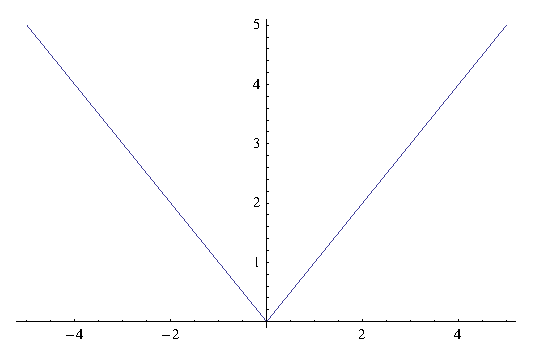
\includegraphics[width=0.5\textwidth]{sl1.eps}
\caption{Grafik funnkcije $f(x) = |x|$}
\end{center}
%Referenca na \cite{lit1}
\end{figure}

\par Zatim nacrtajmo sada grafik funkcije $|x-3|$, dobijamo kada pomerimo grafik udesno za 3 mesta po x-osi.

\begin{figure}[h!]
\begin{center}
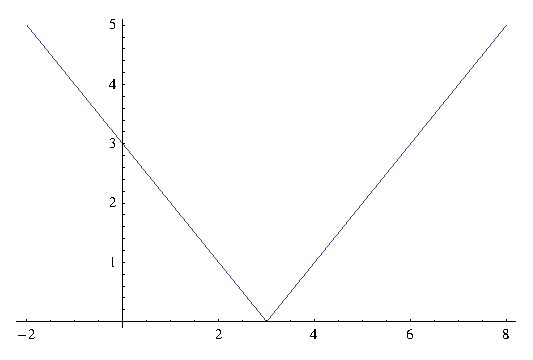
\includegraphics[width=0.5\textwidth]{sl2.eps}
\caption{Grafik funnkcije $f(x) = |x-3|$}
\end{center}
\end{figure}

\par Zatim nacrtajmo sada grafik funkcije $|x-3 | - 1$, dobijamo kada pomerimo grafik nadole za 1 mesto po y-osi.
\begin{figure}[h!]
\begin{center}
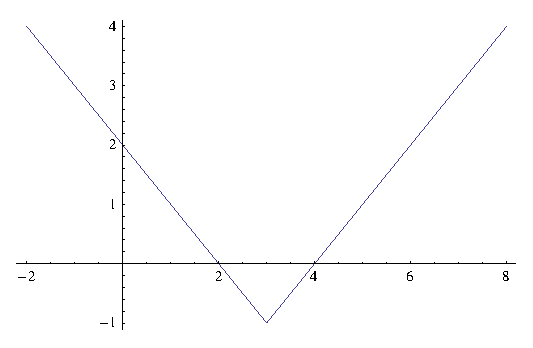
\includegraphics[width=0.5\textwidth]{sl3.eps}
\caption{Grafik funnkcije $f(x) = |x-3| -1$}
\end{center}
\end{figure}
\newpage
\par Zatim nacrtajmo apsolutnu vrednost gornje funkcije to jest nacrtajmo $||x-3 | - 1|$, to se radi tako shto se sve ono shto je ispod x-ose simetrichno preslika iznad nje.
\begin{figure}[h!]
\begin{center}
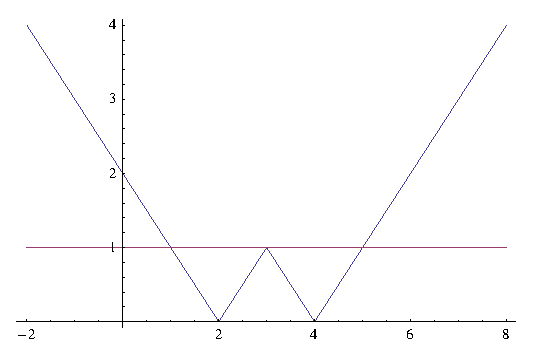
\includegraphics[width=0.5\textwidth]{sl4.eps}
\caption{Grafik funnkcije $f(x) =| |x-3| -1|$}
\end{center}
\end{figure}

\par Sa slike vec1 uochavamo da je reshenje prava $y = 1$, jer jedino ona seche grafik u tachno 3 tachke. To jest reshenje parametra $a$ je 1. \textbf{Odgovor je pod $C$.}

\item Krenemo od $f(x) = \frac{ax +b}{cx+d} $ i zamenjujemo redom vrednosti $x$, i gledamo shta nam to rec1i o funkciji $f$.
\par $f(0) = 1 \Longrightarrow f(0) = \frac{a \cdot 0 + b}{c \cdot 0 + d} = \frac{b}{d} = 1  \Longrightarrow  b = d$. Te znamo da je funckija $f(x)$ oblika $\frac{ax+b}{cx+b}$. Zatim,
\par $f(1) = 0 \Longrightarrow f(1) = \frac{a \cdot 1 + b}{c \cdot 1 + b} = \frac{a+b}{c+b} = 0  \Longrightarrow  a+b = 0$ to jest $a = -b$. Te dobijamo da je funckija $f(x)$ oblika $\frac{-bx+b}{cx+b}$. A iz
\par $f(2) = 3 \Longrightarrow f(2) = \frac{-b \cdot 2 + b}{c \cdot 2 + b} = \frac{-b}{2c+b} = 3  \Longrightarrow  -b = 3 \cdot (2c+b)$, naravno za $2c+b \neq 0$, dobijamo da je $-b = 6c +3b \Longrightarrow c = - \frac{2}{3} b$.
\par Iz svegda ovoga zakljuchujemo daje fukcija $f(x)$ oblika $\frac{-bx + b}{- \frac{2}{3} b x + b} $, kada podelimo brojilac i imenilac sa $b$ dobijamo da je $f(x) =\frac{-x + 1}{- \frac{2}{3} x + 1} =\frac{1-x}{1- \frac{2}{3} x }  $.
\par Odatle mozhemo da izrachunamo $f(3) =\frac{1-3}{1- \frac{2}{3} \cdot 3 } = \frac{-2}{1-2} = 2 $. \textbf{Odgovor je pod $D$.}


%12
\item Pogledajmo prvo sistem:
\begin{center}
\par $(x^{2} - 1)(2x -3y + 4z) = 0$
\par $4x + 5y +8z = -2$
\par $3x + y + 6z = 44$
\end{center}

\par Lichi na sistem 3 jednachine sa 3 nepoznate, samo shto nam smeta $(x^{2} - 1)$  iz prve jednachine. Pa hajdemo da se reshimo toga. Kada je $x^{2} - 1 = 0$ to jest kada je $x^{2} =1$, ochigledno je za $x = \pm 1$.
\par Razmatrac1emo tri sluchaja kada je $x = 1$, $x+ -1$ i kada je $x \neq \pm 1$.
\begin{enumerate}[1)]

\item Kada je $x = 1$ dobijamo sistem:
\begin{center}
\par $4 + 5y +8z = -2$
\par $3 + y + 6z = 44$
\end{center}
\begin{center}
\par $5y +8z = -6$
\par $y + 6z = 41$
\end{center}
\par Izrazimo sada $y$:
\begin{center}
\par $5y +8z = -6$
\par $y = 41 - 6z$
\end{center}
\par Zamenimo $y$ u gornju jednachinu:
\begin{center}
\par $5 \cdot (41 - 6z) +8z = -6$
\par $y = 41 - 6z$
\end{center}
\begin{center}
\par $205 -30z +8z = -6$
\par $y = 41 - 6z$
\end{center}
\begin{center}
\par $-22z = -211$
\par $y = 41 - 6z$
\end{center}
\par Izrachunajmo sada $z$:
\begin{center}
\par $z = \frac{211}{22}$
\par $y = 41 - 6z$
\end{center}
\par Zamenimo vrednost $z$ u donji izraz da bismo dobili $y$:
\begin{center}
\par $z = \frac{211}{22}$
\par $y = 41 - 6 \cdot \frac{211}{22} = - \frac{182}{11}  $
\end{center}
\par Te je reshenje sistema jedinstveno i glasi $(1,-\frac{182}{11}, \frac{211}{22})$.

\item Kada je $x = -1$ dobijamo sistem:
\begin{center}
\par $-4 + 5y +8z = -2$
\par $-3 + y + 6z = 44$
\end{center}
\begin{center}
\par $5y +8z = 2$
\par $y + 6z = 47$
\end{center}
\par Izrazimo sada y:
\begin{center}
\par $5y +8z = 2$
\par $y = 47 - 6z$
\end{center}
\par Zamenimo $y$ u gornju jednachinu:
\begin{center}
\par $5 \cdot (47 - 6z) +8z = 2$
\par $y = 47 - 6z$
\end{center}
\begin{center}
\par $235-30z +8z = 2$
\par $y = 47 - 6z$
\end{center}
\begin{center}
\par $-22z=-233$
\par $y = 47 - 6z$
\end{center}
\begin{center}
\par $z = \frac{233}{22}$
\par $y = 47 - 6z$
\end{center}
\par Zamenimo vrednost $z$ u donji izraz da bismo dobili $y$:
\begin{center}
\par $z = \frac{233}{22}$
\par $y = 47 - 6 \cdot \frac{233}{22} = - \frac{182}{11}$
\end{center}
\par Te je reshenje sistema jedinstveno i glasi $(1,-\frac{182}{11}, \frac{211}{22})$.

\item Poshto je $x \neq \pm 1$, onda prvu jednachinu mozhemo podeliti sa $(x^2 - 1)$, i reshavamo sistem:
\begin{center}
\par $2x -3y + 4z = 0$
\par $4x + 5y +8z = -2$
\par $3x + y + 6z = 44$
\end{center}
\par Ovaj sistem je 3x3 pa se malo tezhe reshava. Mozhemo uochiti linearnu zavisnost jednachina i lako je pokazati. Pomnozhimo prvu jednachinu sa -2 i dodamo je drugoj, i sa $-\frac{3}{2}$ i dodamo je trec1oj. Time dobijamo:
\begin{center}
\par $2x -3y + 4z = 0$
\par $11y = -2 \Longrightarrow y = -\frac{11}{2}$
\par $\frac{11}{2}y = 44 \Longrightarrow y = 8$
\end{center}
\par Ovime smo dobili kontradikciju, to jest da ovaj sistem nema reshenje.
\end{enumerate}
\par Zakljuchak je da polazni sistem ima samo dva reshenja. \textbf{Odgovor je pod $C$.} 

\textbf{Ubaciti laksi nacin resavanja ovog zadataka, bez bukvalnog racunanja}

\item Pogledajmo polazni sistem:
\begin{center}
\par $7 \cdot 3^{x} - 5 \cdot 2^{y} = 23$
\par $2 \cdot 3^{x} + 3 \cdot 2^{y} = 42$
\end{center}
\par Uvodimo smenu $a = 3^x, b = 2^y$, tada nam sistem izgleda:
\begin{center}
\par $7 a - 5b = 23$
\par $2 a + 3 b = 42$
\end{center}
\par Ovo je sistem linearnih jednachina sa dve nepoznate koji se jako lako reshi, i njegova reshenja su:
\begin{center}
\par $a = 9$
\par $b = 8$
\end{center}
\par Pa je reshenje polaznog sistema:
\begin{center}
\par $3^x = a = 9\Longrightarrow x = 2$
\par $2^y = b = 8 \Longrightarrow y = 3$
\end{center}
\par Trazheni izraz $x+y = 5$. \textbf{Odgovor je pod $E$.}

\item Da bismo ovo reshili treba da znamo svojstva logaritma. Ona koja su nam ovde potrebna su: $\log_{a^n} b = \frac{1}{n} \log_a b$, $\log_a b^n = n \log_a b$, $\log_a a = 1$ i  $\log_a b + \log_a c = \log_a bc$.
\begin{center}
\par $ \log_{36} x^{2} + \log_6 (x + 5) -1 = 0$
\par $ \log_{6^2} x^{2} + \log_6 (x + 5) = 1$
\par $ \frac{1}{2} \log_6 x^{2} + \log_6 (x + 5) = 1$
\par $ \frac{1}{2} \cdot 2 \cdot \log_6 |x| + \log_6 (x + 5) = 1$
\end{center}
\par Ovde mora $|x|$ jer nije naznacheno koji je domen u pitanju.
\begin{center}
\par $ \log_6 |x| + \log_6 (x + 5) = 1$
\par $ \log_6 |x|(x + 5) = 1$
\par $ \log_6 |x|(x + 5) = \log_6 6$
\par $|x|(x + 5) = 1$
\end{center}
\par Razmatramo sada dva sluchaja:
\begin{enumerate}[1)]
\item Kada je $x > 0$: $x(x+5) = 6 \Longrightarrow x^2 + 5x -6 = 0 \Longrightarrow (x+6)(x-1)=0$. Reshenje za ovaj sluchaj je $x = 1$.
 
\item Kada je $-5 < x < 0$:  $-x(x+5) = 6 \Longrightarrow -x^2 - 5x -6 = 0 \Longrightarrow -(x+3)(x+2)=0$. Reshenja za ovaj sluchaj je $x = -2$ i  $x = -3$.
\par Napomena: Kada je logaritam u pitanju, ono shto je pod njim ne sme biti 0, stoga se samo razmatra kada je $x$ manje od 0. Takodje gore imamo $\log_6 (x+5)$ odakle uzimamo drugo ogranichenje a to je da $x+5>0$ to jest $ x > -5$.
\end{enumerate}
\par Proizvod reshenja je $1 \cdot (-2) \cdot (-3) = 6$. \textbf{Odgovor je pod E.} 


\item Posmatrajmo prvo interval od $[0,\pi]$. Na intervalu $\left[0, \frac{\pi}{4}\right)$ je, $\sin x < \cos x$, a na intervalu $\left(\frac{3\pi}{4}, \pi\right]$ je $\sin x < |\cos x|$, dok na ostalim delovim u okviru $[0,\pi]$ uslov nije ispunjen.
\par Kada imamo to uocheno razmotrimo sada neke aproksimacije koje c1e nam pomoc1i za dalje razmatranje: $\frac{\pi}{4} = 0.735
$, $\frac{3\pi}{4} = 2.305$, $\pi = 3.14$, $2\pi = 6.28$, $2\pi + \frac{\pi}{4} =\frac{9\pi}{4} = 7.015$, $2\pi + \frac{3\pi}{4} =\frac{11\pi}{4} = 8,585$, $3\pi = 9.42$.
\begin{itemize}
\item $x \in \left[0,\frac{\pi}{4}\right)\rightarrow $ reshenje je 0.
\item $x \in \left(\frac{3\pi}{4}, \pi\right] \rightarrow $ reshenje je 3.
\item $x \in [\pi, 2\pi) \rightarrow $ reshenja su 4,5,6.
\item $x \in \left[2\pi, \frac{9\pi}{4}\right) \rightarrow $ reshenje je 7.
\item $x \in \left(\frac{11\pi}{4}, 3\pi\right] \rightarrow $ reshenja nema, jer je ovo disjunktno sa $[0,8]$.
\end{itemize}
\par Broj reshenja je 6. \textbf{Odgovor je pod $C$.} 


%16,17,18
\item Trougao $\triangle MNP$ je jednakostranichni, pa je dovoljno izrachunati njegovu stranicu. Iskoristimo dva puta Pitagorinu teoremu. Iz pravouglog trougla $\triangle MBC$ sledi da je $MC^2=MB^2+BC^2=2^2+4^2=20$, a iz pravouglog trougla $\triangle MCN$ sledi da je $MN^2=MC^2+CN^2=20+2^2=24$. Prema tome, povrshina trougla $\triangle MNP$ je $\frac{MN^2\sqrt{3}}{4}=\frac{24\sqrt{3}}{4}=6\sqrt{3}$. \textbf{Odgovor je pod $E$.}


\begin{figure}[h!]
\begin{center}
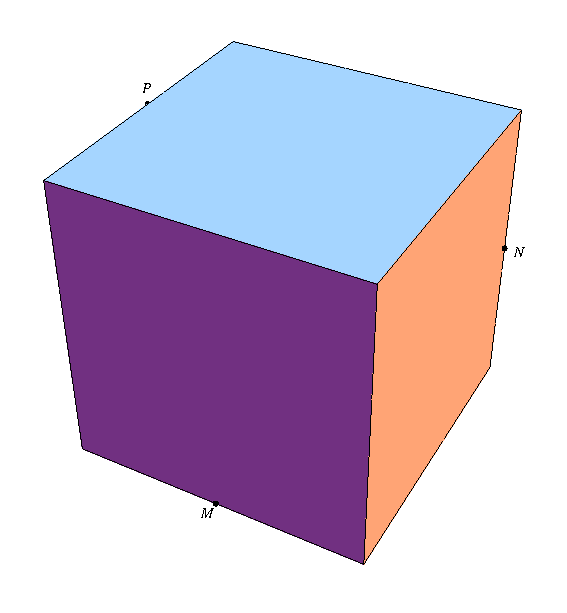
\includegraphics[width=0.5\textwidth]{sl5.eps}
\caption{Slika uz zadatak}
\end{center}
\end{figure}

\item Izdelimo chetvorougao na 8 trouglova: $\triangle AMS$, $\triangle BMS$, $\triangle BNS$, $\triangle CNS$, $\triangle CPS$, $\triangle DPS$, $\triangle DQS$, $\triangle AQS$.
\begin{figure}[h!]
\begin{center}
\includegraphics[width=0.4\textwidth]{sl8.eps}
\caption{Slika uz zadatak}
\end{center}
\end{figure}
Zbir povrshina ovih trouglova jednak je povrshini chetvorougla $ABCD$, dakle $90\mathrm{\ cm}^2$. Ovi trouglovi su pravougli i svima je kateta koja sadrzhi teme $S$ jednaka poluprechniku $r$ upisane kruzhnice. Oznachimo $AM=AQ=x$, $BM=BN=y$, $CN=CP=z$, $DP=DQ=t$ (tangentne duzhi iz iste tachke su jednake). Tada je:
\par $90=\frac{r \cdot x}{2}+\frac{r \cdot y}{2}+\frac{r \cdot y}{2}+\frac{r \cdot y}{2}+\frac{r \cdot z}{2}+\frac{r \cdot z}{2}+\frac{r \cdot t}{2}+\frac{r \cdot t}{2}=\frac{r}{2}\cdot(2x+2y+2z+2t)=r\cdot(x+y+z+t)$.
\par Primetimo da je $x+y+z+t=AB+CD=15$, pa je $90=r\cdot 15$, odakle sledi da je $r=6\mathrm{\ cm}$. \textbf{Odgovor je pod $A$.}

\item Neka je $R$ poluprechnik vec1eg, a $r$ poluprechnik manjeg kruga. Tetiva $AB$ je tangenta na manji krug, pa sledi da je u dodirnoj tachki $S$ normalna na poluprechnik $OS$. Poshto je $OA=OB=R$, sledi da je trougao $\triangle OAB$ jednakokraki. Prema tome, $S$ je sredishte stranice $AB$.
\begin{figure}[h!]
\begin{center}
\includegraphics[width=0.4\textwidth]{sl7.eps}
\caption{Slika uz zadatak}
\end{center}
\end{figure}
U pravouglom trouglu $\triangle SOA$ imamo da je $OA^2=OS^2+SA^2$ na osnovu Pitagorine teoreme, tj. $R^2=3^2+r^2$. Dakle, $R^2-r^2=9$. Povrshina kruzhnog prstena jednaka je $R^2\pi-r^2\pi$, pa sledi da je jednaka $9\pi$. \textbf{Odgovor je pod $B$.}

\item Pogledajmo jednachine pravih $2x + y - 3 = 0$, $2x +y -8 = 0$. Zapishimo ih malo drugachije $y = -2x +3$, $y=  2x + 8$. Vidimo da su koeficijenti pravca jednaki te da su prave paralelne. Da bismo dobili ivicu kvadrata dovoljno je naci rastpojanje imedju pravih. To c1emo nac1i tako shto c1emo uzeti neku tachku sa jedna prave, i nac1i njeno rastojanje od druge prave.
\par Uzec1u tachku sa prve prave, i neka to bude tachka u kojoj $x$ uzima vrednost 0. To c1e biti tachka gde je $y = -2 \cdot 0 +3 = 3$, to jest tachka $(0,3)$. Koristec1i formulu za nalazhenje odstojanaj tachke od prave nalazimo ivicu kvadrata $a$: (Neka je prava $q$ zadata jednachinom $ 2x+y-8 = 0$)
\par $d((0,3), q) = \frac{|2 \cdot 0 + 1 \cdot 3 -8|}{\sqrt{2^2 + 1^2}} = \frac{|-5|}{\sqrt{5}} = \sqrt{5}$
\par Dobijemo da je $a = \sqrt{5}$ to jest povrshina kvadrata je 5. \textbf{Odgovor je pod $B$.} 


\item Kako imamo $a,b,\sin{\alpha} $ mozhemo koristec1i sinusnu teorenu da nadjemo i $\sin{\beta}$:
\par $ \frac{a}{\sin{\alpha}}= \frac{b}{\sin{\beta}}  \Longrightarrow \frac{60}{\frac{12}{13}}= \frac{52}{\sin{\beta}} \Longrightarrow \sin{\beta} = \frac{4}{5} $
\par Kako imamo vrednosti sinusa uglove, mozhemo lako nac1i vrednosti kosinusa iz relacije $\sin^2  x  +\cos^2  x  = 1$, a kako su to uglovi trougla znamo da c1e vrednosti biti pozitivne. Sa lakoc1om nalazimo $\cos{\alpha} = \frac{5}{13}, \cos{\beta} = \frac{3}{5} $.
\par Poshto je $\gamma = \pi - \alpha - \beta$ imamo: 
\par $\sin{\gamma} = \sin(\pi - \alpha - \beta)= \sin( \alpha + \beta) = \sin{\alpha}\cos{\beta} + \sin{\beta} \cos{\alpha} = \frac{12}{13}\cdot \frac{3}{5} + \frac{5}{13}  \cdot \frac{4}{5} = \frac{36+20}{65} = \frac{56}{65} $. \textbf{Odgovor je pod $A$.}


\end{enumerate}
\newpage



\begin{thebibliography}{9}
%Literatura

\bibitem{lit1} Ognjanovic1 Srdjan, {\it Matematika {\Lat 4+}}, Krug Beograd
\bibitem{lit2} \href{https://www.wolframalpha.com/}{Volfram alfa} - za proveru rechuna
\bibitem{lit3} \href{http://www.matf.bg.ac.rs/files/prijemni_jun_2016_.pdf}{Zadaci sa prijemnog}

\end{thebibliography}

\end{document}